\documentclass[../main.tex]{subfiles} % required, if the Chapter be a seperate doc

\begin{document}

\section{Statistik}\label{sec:statistik}
\subsection{Feder 1}\label{subsec:statik-feder-1}
\begin{figure}[H]
    \centering
    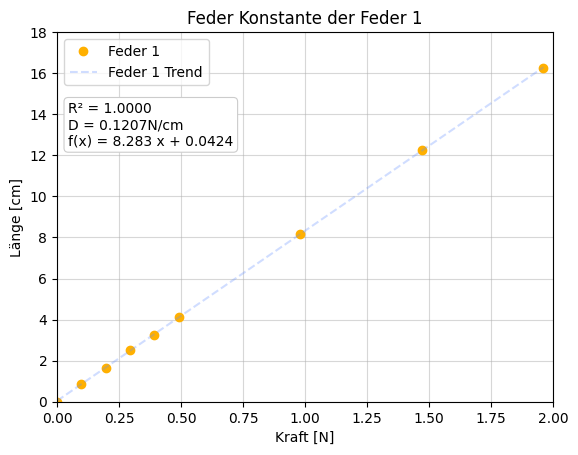
\includegraphics[scale=0.5]{graph/Spring-1}
    \caption{Graph von den gemessenen Werte von Feder 1 dargestellt und darstellung der Trendline}
    \label{fig:graph-spring-1}
\end{figure}
\subsection{Feder 2}\label{subsec:statik-feder-2}
\begin{figure}[H]
    \centering
    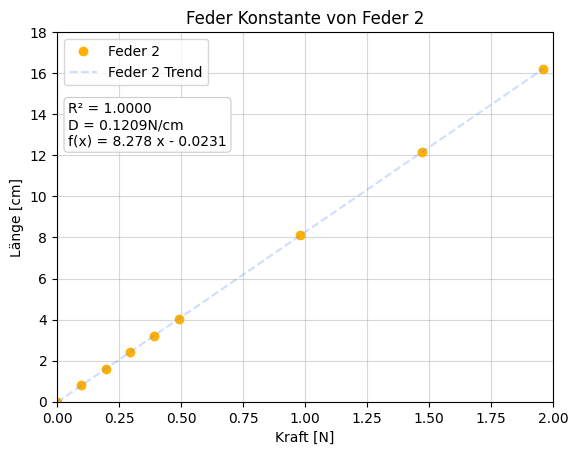
\includegraphics[scale=0.5]{graph/Spring-2}
    \caption{Graph von den gemessenen Werte von Feder 2 dargestellt und darstellung der Trendline}
    \label{fig:graph-spring-2}
\end{figure}
\subsection{Seriell}\label{subsec:statik-spring-series}
\begin{figure}[H]
    \centering
    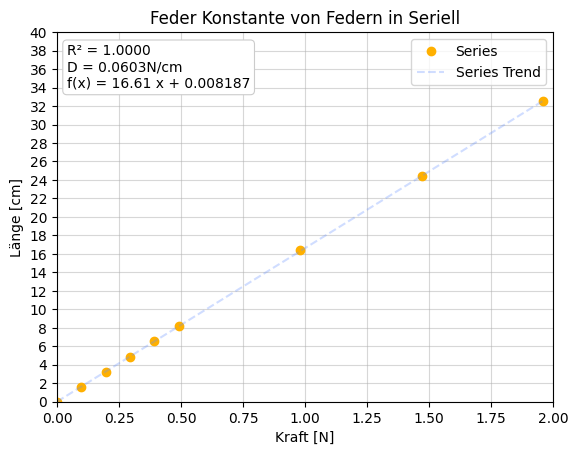
\includegraphics[scale=0.5]{graph/Spring-Series}
    \caption{Graph von den gemessenen Werte von Feder in Serieller Anordnung dargestellt mit darstellung der Trendline}
    \label{fig:graph-spring-series}
\end{figure}
\subsection{Parallel}\label{subsec:statik-spring-parallel}
\begin{figure}[H]
    \centering
    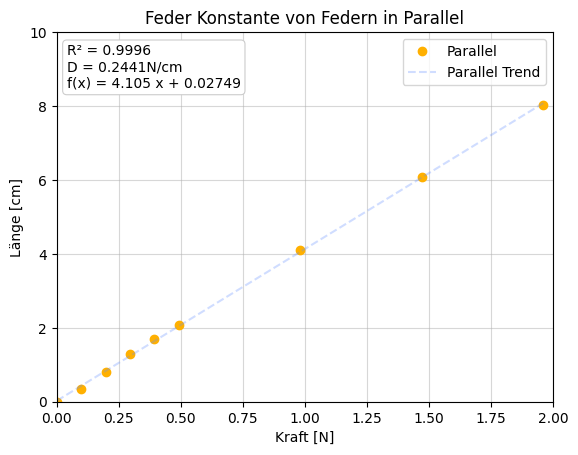
\includegraphics[scale=0.5]{graph/Spring-Parallel}
    \caption{Graph von den gemessenen Werte von Feder in Paralleler Anordnung dargestellt mit darstellung der Trendline}
    \label{fig:graph-spring-parallel}
\end{figure}
\subsection{Feder Vergleiche}\label{subsec:statik-spring-comparisons}
\begin{figure}[H]
    \centering
    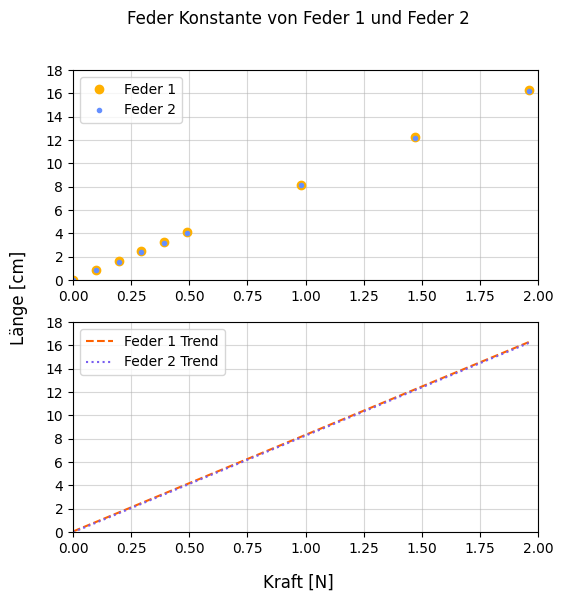
\includegraphics[scale=0.7]{graph/Spring-1-and-Spring-2}
    \caption{Die Darstellung der beiden gemessenen Federn übereinander gesetzt mit Datenpunkte und Trendlinie}
    \label{fig:graph-single-spring-comparisons}
\end{figure}
\end{document}